\documentclass[12pt]{article}

\usepackage[margin=2cm]{geometry}   

\usepackage{amsfonts}

\usepackage{tikz}
\usetikzlibrary{shapes,arrows}
\usetikzlibrary{positioning}

\begin{document}




% Define block styles
\tikzstyle{space} = [ellipse, draw=black, minimum width=25mm, minimum height=15mm]
 

\begin{tikzpicture}[node distance=2cm]

    % Place nodes
    \node [space] [label=Sample Space] (sample) {$\Omega$} ;
    \node [space, right= of sample] [label=Random Variable] (rv) {$\mathbb{R}$};
    \node [space, right= of rv] (density) [label=Probability Density] {$[0, \infty)$};
    \node [space, right= of density] (prob) [label=Probability] {$[0, 1]$};

    % Draw edges
    \draw [->] (sample) -- (rv) node [midway, above] {$X$};
    \draw [->] (rv) -- (density) node [midway, above] {$f$};
    \draw [->] (density) -- (prob) node [midway, above] {$\int f dx$};

\end{tikzpicture}


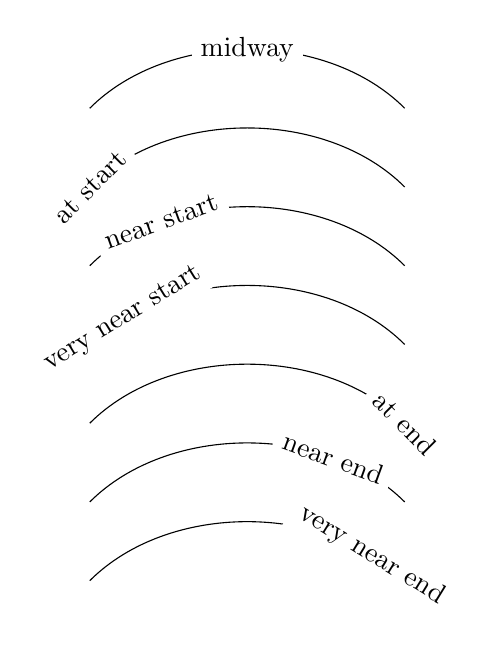
\begin{tikzpicture}
\foreach \x [count=\i] in {midway, at start, near start, very near start, at end, near end, very near end} {
  \draw (0,-\i) .. controls ++(1,1) and ++(-1,1) .. ++(4,0) node [\x, sloped, fill=white] () {\x};
}
\end{tikzpicture}

\end{document}
